\documentclass[a4paper]{article}
 
% - taille de la fonte    : 10pt, 11pt, 12pt
% - recto ou recto-verso    : oneside, twoside
 
% Chargement d'extensions
%\usepackage[latin1]{inputenc}    
\usepackage[francais]{babel}    
\AtBeginDocument{\def\labelitemi{$\bullet$}}

\usepackage{amsmath}
\makeatletter
%%%%%%%%%%%%%%%%%%% debut fichier boiboites.sty %%%%%%%%%%%%%%%%%%%%%%
\RequirePackage{xkeyval}
\RequirePackage{tikz}
\RequirePackage{amssymb}

\define@key{boxedtheorem}{titlecolor}{\def\titlecolor{#1}}
\define@key{boxedtheorem}{titlebackground}{\def\titlebackground{#1}}
\define@key{boxedtheorem}{background}{\def\background{#1}}
\define@key{boxedtheorem}{titleboxcolor}{\def\titleboxcolor{#1}}
\define@key{boxedtheorem}{boxcolor}{\def\boxcolor{#1}}
\define@key{boxedtheorem}{thcounter}{\def\thcounter{#1}}
\define@key{boxedtheorem}{size}{\def\size{#1}}
\presetkeys{boxedtheorem}{titlecolor = black, titlebackground = white, background = white,%
                         titleboxcolor = black, boxcolor = black, thcounter=, size = .9\textwidth}{}

\newcommand{\couleurs}[1][]{%
    \setkeys{boxedtheorem}{#1}
    \tikzstyle{fancytitle} =[draw=\titleboxcolor, rounded corners, fill=\titlebackground,
                            text= \titlecolor]
    \tikzstyle{mybox} = [draw=\boxcolor, fill=\background, very thick,
                        rectangle, rounded corners, inner sep=10pt, inner ysep=20pt]
}


%Commande generique pour faire un joli encadre
\newsavebox{\boiboite}
\newcommand{\titre}{Titre}
\newenvironment{boite}[2][]%
    {%
    \renewcommand{\titre}{#2}
    \couleurs[#1]
    \begin{lrbox}{\boiboite}%
     \begin{minipage}[!h]{\size}
    }%
    {%
     \end{minipage}
    \end{lrbox}
    \begin{center}
    \begin{tikzpicture}
    \node [mybox] (box){\usebox{\boiboite}};
    \node[fancytitle, right=10pt] at (box.north west) {\titre};
    \end{tikzpicture}
    \end{center}
    }

\newcommand{\newboxedtheorem}[4][]{%
    \couleurs[#1]
    \@ifnotempty{#4}{%
      \@ifundefined{the#4}{\@ifundefined{\thcounter}{\newcounter{#4}}{%
      \newcounter{#4}[\thcounter ] } } { }%
    }
    \newenvironment{#2}[1][]{%
    \@ifnotempty{#4}{\refstepcounter{#4}}
    \begin{boite}[#1]{\textbf{#3\@ifnotempty{#4}{ \csname the#4\endcsname}}\@ifnotempty{##1}{
    (##1)}}
    }%
    {%
    \end{boite}
    }
}
%%%%%%%%%%%%%%%%%%%% end fichier boiboites.sty %%%%%%%%%%%%%%%%%%%%%%
\makeatother
\newboxedtheorem{theorem}{}{theorem}
%%%%%%%%%% hypertext

\usepackage{hyperref}
\hypersetup{
    colorlinks=true,
    linkcolor=blue,
    filecolor=magenta,      
    urlcolor=cyan,
    pdftitle={Overleaf Example},
    pdfpagemode=FullScreen,
    }

\urlstyle{same}

%%%%%%%%%%%%%%%%%%%%%%%%%%%
\usepackage{amsthm}
%\usepackage{amsmath}
\usepackage{amssymb}
\usepackage{mathrsfs}
\usepackage{graphicx}
\usepackage{geometry}
\usepackage{stmaryrd}
\usepackage{tikz}
\usetikzlibrary{patterns}

\usepackage[cache=false]{minted}
\usepackage{xcolor}
%\setbeamercolor{background canvas}{bg=lightgray}
\definecolor{LightGray}{gray}{0.9}
\definecolor{monOrange}{rgb}{0.97,0.35,0.04}

% Informations le titre, le(s) auteur(s), la date
\title{Rendez vos endpoints plus performants}
\author{Ibrahim ALAME}
\date{\today}
\includeonly{ introduction.tex} 
\begin{document}
 
\maketitle
 %Mettez en place une API simple avec Django REST Framework
\section{Minimisez les appels de votre API grâce aux serializers}
\subsection{Retournez plus d'informations}
En l’état, les clients (application front, mobile, etc.) de notre API doivent réaliser {\em plusieurs appels} pour obtenir la liste des catégories et la liste des produits qui composent chacune d’entre elles.
\begin{center}
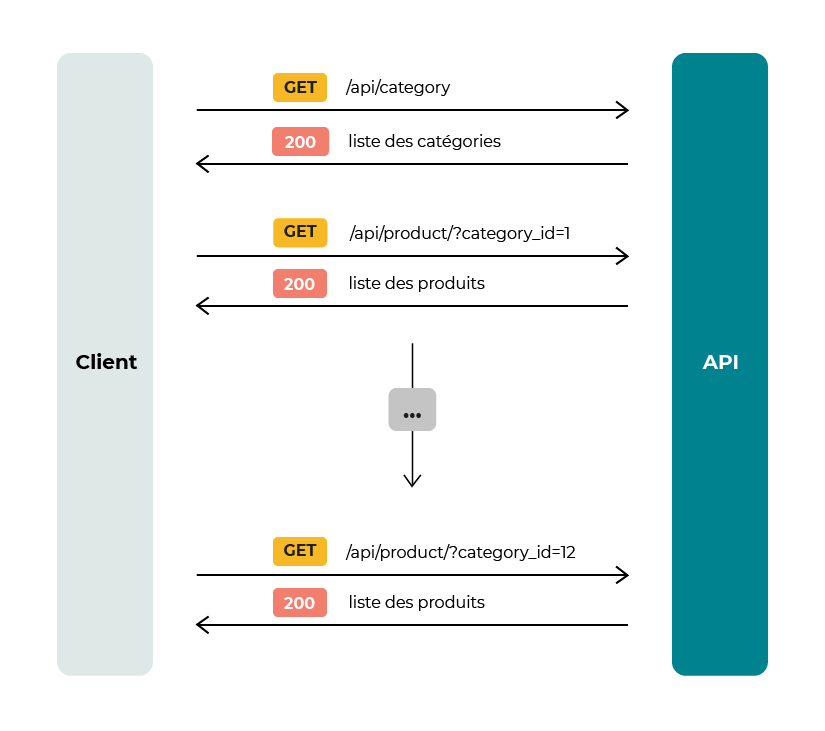
\includegraphics[width=12cm]{images/image11.png}
\end{center}
Donc autant d’appels qu’il y a de catégories sont nécessaires, ce qui n’est pas très optimal. Pour résoudre cette problématique, il est possible d’{\em imbriquer des serializers}, afin que le serializer des catégories renvoie directement la liste des produits qui composent la catégorie consultée. Et c’est ce que nous allons voir tout de suite ensemble.
\begin{theorem}
Attention tout de même à ne pas imbriquer trop de serializers car beaucoup d’appels en base de données peuvent être faits, à moins d’optimiser ces appels à l’aide de {\tt prefetch\_related}  et de {\tt select\_related} . Certains calculs de valeurs d’attributs peuvent aussi être coûteux, il faut donc utiliser l’imbrication avec parcimonie, selon les cas qui se présentent à nous.
\end{theorem}
\subsection{Imbriquez les serializers}
Nous allons faire en sorte que notre endpoint de catégorie renvoie également la liste des produits qui le composent. Pour cela, {\em éditons notre serializer de catégorie} en ajoutant dans la liste des fields le {\tt related\_name}  vers les produits définis dans notre model :
\begin{minted}[
mathescape,
framesep=2mm,
baselinestretch=1.2,
%fontsize=\footnotesize,
bgcolor=LightGray,
%linenos
]{python}
class CategorySerializer(ModelSerializer):
 
class Meta:
model = Category
        fields = ['id', 'date_created', 'date_updated', 'name', 'products']
\end{minted}
\begin{theorem}
Lorsque nous ajoutons un {\tt related\_name}  dans un serializer, DRF va ajouter la liste des identifiants distants dans un attribut portant le même nom que le {\tt related\_name}.
\end{theorem}

\begin{center}
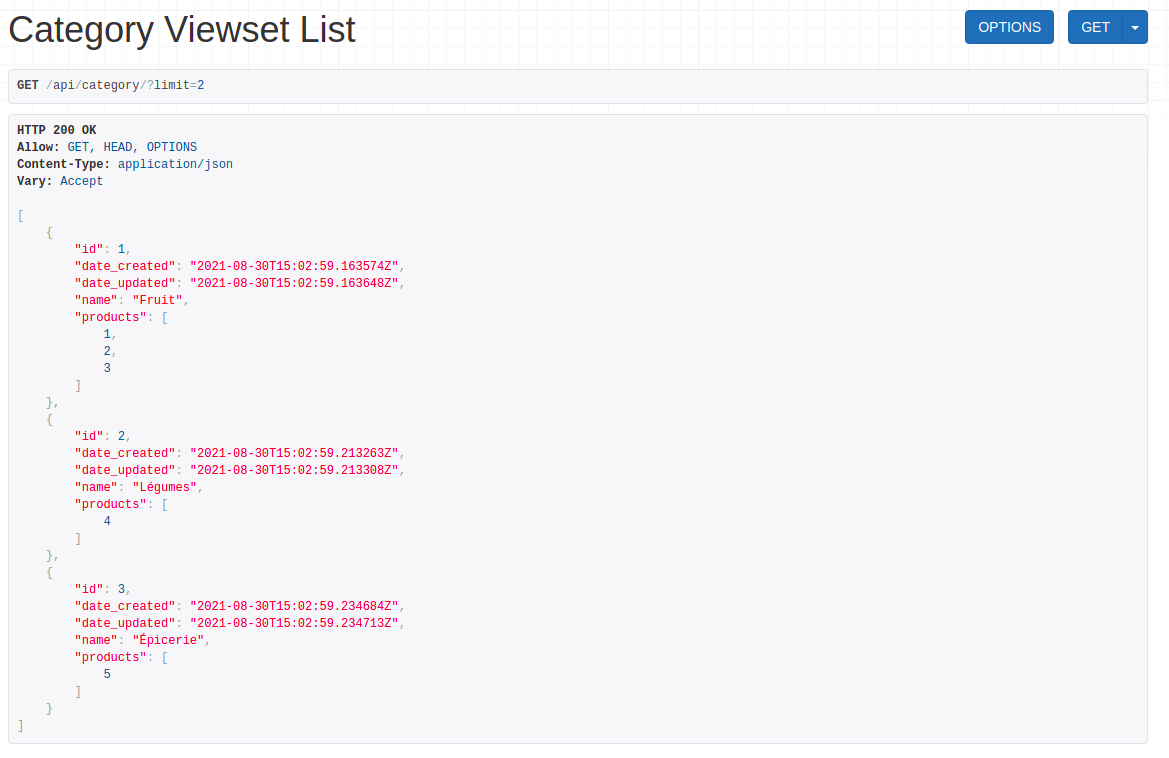
\includegraphics[width=12cm]{images/image12.png}
\end{center}

Cependant, un problème persiste, DRF affiche tous les produits de chaque catégorie, alors que nous voudrions n'afficher que ceux qui sont {\em actifs}. Pour cela, nous pouvons redéfinir notre attribut de classe {\tt products}  avec un {\tt SerializerMethodField}  qui nous donne alors la possibilité de {\em filtrer les produits à retourner}.
\begin{minted}[
mathescape,
framesep=2mm,
baselinestretch=1.2,
fontsize=\footnotesize,
bgcolor=LightGray,
%linenos
]{python}
class CategorySerializer(serializers.ModelSerializer):

    # En utilisant un `SerializerMethodField', il est nécessaire d'écrire une méthode
    # nommée 'get_XXX' où XXX est le nom de l'attribut, ici 'products'
    products = serializers.SerializerMethodField()

    class Meta:
        model = Category
        fields = ['id', 'date_created', 'date_updated', 'name', 'products']

    def get_products(self, instance):
        # Le paramètre 'instance' est l'instance de la catégorie consultée.
        # Dans le cas d'une liste, cette méthode est appelée autant de fois qu'il y a
        # d'entités dans la liste

        # On applique le filtre sur notre queryset pour n'avoir que les produits actifs
        queryset = instance.products.filter(active=True)
        # Le serializer est créé avec le queryset défini et toujours défini en tant que many=True
        serializer = ProductSerializer(queryset, many=True)
        # la propriété '.data' est le rendu de notre serializer que nous retournons ici
        return serializer.data
\end{minted}

\begin{center}
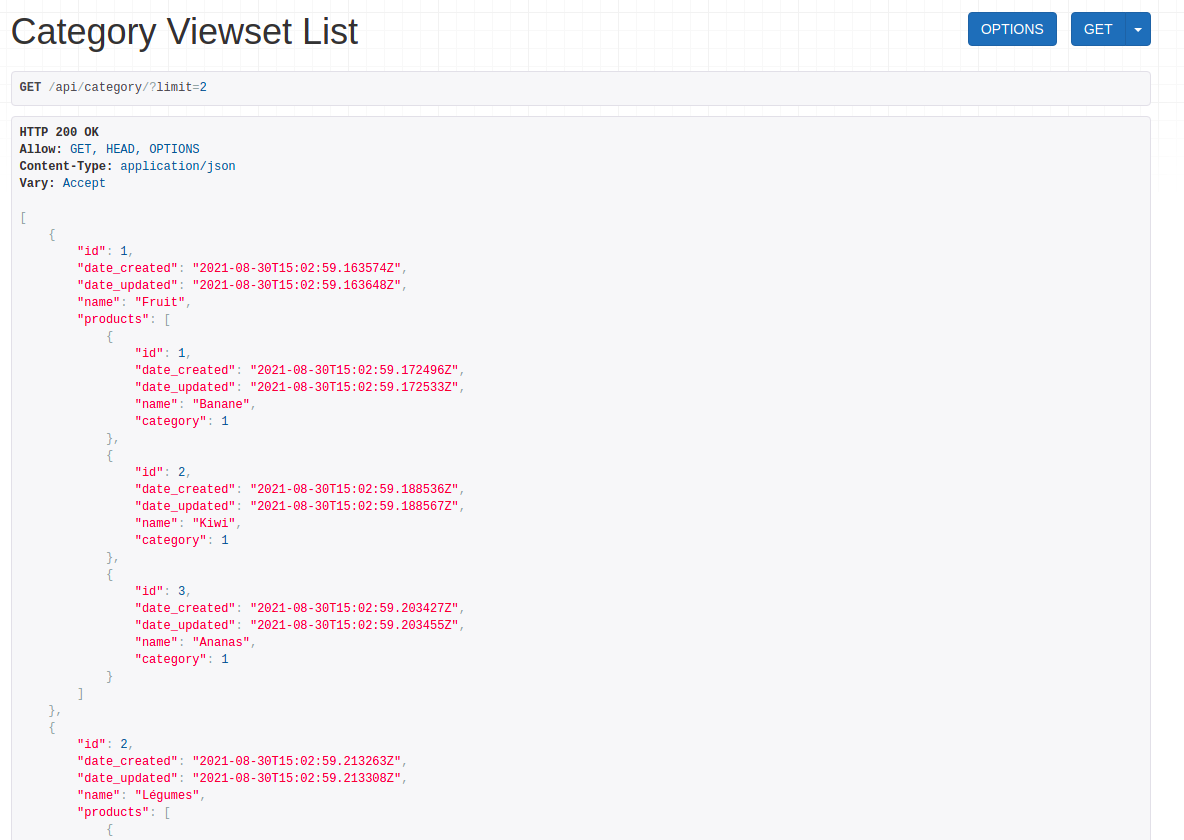
\includegraphics[width=12cm]{images/image13.png}
\end{center}
Nous pouvons constater qu'à présent les produits retournés sont bien seulement des produits actifs.

\subsubsection*{Et si on lançait nos tests après le développement de cette feature ?}
Oups, c’est cassé ! Et c’est tout à fait {\color{monOrange}normal}.

Une API se doit d’être minutieusement {\color{monOrange}testée}, car les retours de ces endpoints sont souvent garants du bon fonctionnement des applications clientes. L’ajout d’un attribut dans un endpoint ne pose en général aucun problème, mais le {\color{monOrange}retrait} d’un attribut peut avoir des conséquences plus importantes.

Imaginons que l’application mobile de notre site utilise l’attribut price  de nos articles, et que nous décidions de le {\color{monOrange}retirer} pour le déplacer ailleurs. Les applications mobiles ne pourraient pas alors afficher de prix tant qu’ils ne déploient pas eux-mêmes une nouvelle version de leur application qui utilise le {\color{monOrange}nouvel attribut}.

\subsubsection*{Mais ça fait beaucoup de données tout ça pour un seul endpoint, non ?}
Pour limiter les données retournées, il est possible de mettre en place une {\color{monOrange}pagination}. Faisons-le ensemble !
\subsection{Ajoutez de la pagination}
Mettre en place une pagination dès la création d’une API est une bonne pratique, car en limitant le nombre d’entités retournées, cela permet :
\begin{itemize}
\item De réduire le temps de réponse, surtout si le calcul de certains attributs est coûteux ;
\item Aux applications clientes de ne pas récupérer toutes les informations si elles ne se servent que d’une seule partie ;
\item D’éviter la modification des applications clientes par la suite, car la pagination impose certains attributs.
\end{itemize}
Il suffit d'jouter dans {\tt settings.py}:
\begin{minted}[
mathescape,
framesep=2mm,
baselinestretch=1.2,
fontsize=\footnotesize,
bgcolor=LightGray,
%linenos
]{python}
REST_FRAMEWORK = {
   'DEFAULT_PAGINATION_CLASS':
   'rest_framework.pagination.LimitOffsetPagination',
   'PAGE_SIZE': 10
}
\end{minted}

\begin{center}
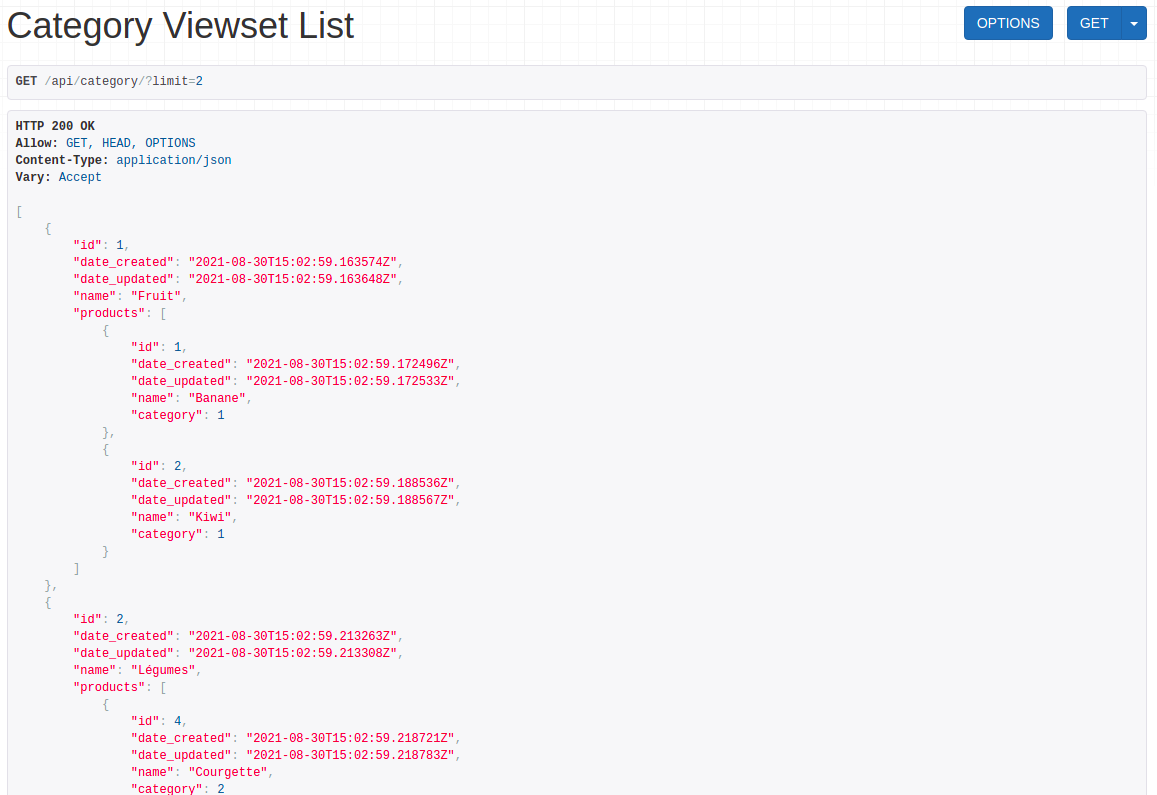
\includegraphics[width=12cm]{images/image14.png}
\end{center}
La pagination indique les informations suivantes :
\begin{itemize}
\item {\tt count  :} le nombre total d’éléments ;
\item {\tt next  :} l’URL de l’endpoint pour obtenir la page suivante ;
\item {\tt previous  :} l’URL de l’endpoint pour obtenir la page précédente ;
\item {\tt results  :} les données réelles utilisables.
\end{itemize}
\begin{theorem}
Lorsque les applications clientes sont réalisées en interne, il est important de bien communiquer avec ses équipes afin de savoir quelles sont les données qui leurs sont importantes, et dans quelles conditions. Le résultat de ces échanges vous donnera les meilleures pistes pour savoir quelles données retourner, et sous quel format.
\end{theorem}
Je vous propose de mettre en place le même mécanisme d’imbrication sur le serializer de produits, pour que les applications clientes puissent récupérer d’un coup les produits et leurs articles actifs.

Pour réaliser cela, vous pouvez partir de la branche \href{https://github.com/OpenClassrooms-Student-Center/7192416\_APIs\_DRF/tree/P2C1\_exercice}{P2C1\_exercice}. Elle contient déjà ce que nous venons de faire ensemble. Une solution est proposée sur la branche \href{https://github.com/OpenClassrooms-Student-Center/7192416\_APIs\_DRF/tree/P2C1\_solution}{P2C1\_solution}.
\begin{minted}[
mathescape,
framesep=2mm,
baselinestretch=1.2,
fontsize=\footnotesize,
bgcolor=LightGray,
%linenos
]{python}
from rest_framework import serializers
from shop.models import Category,Product,Article
 
class ArticleSerializer(serializers.ModelSerializer):
    class Meta:
        model = Article 
        fields = ['id', 'date_created', 'date_updated','name','description','active','price']

class ProductSerializer(serializers.ModelSerializer):
    articles=serializers.SerializerMethodField()
    class Meta:
        model = Product
        fields = ['id', 'date_created', 'date_updated','name','category','articles']  
          
    def get_articles(self,instance):
        queryset = instance.articles.filter(active=True)  
        serializer = ArticleSerializer(queryset,many=True) 
        return serializer.data 
         
class CategorySerializer(serializers.ModelSerializer):
    products=serializers.SerializerMethodField()
    class Meta:
        model = Category
        fields = ['id', 'date_created', 'date_updated' ,'name','products']  
    def get_products(self,instance):
        queryset = instance.products.filter(active=True)  
        serializer = ProductSerializer(queryset,many=True) 
        return serializer.data        
\end{minted}
\begin{center}
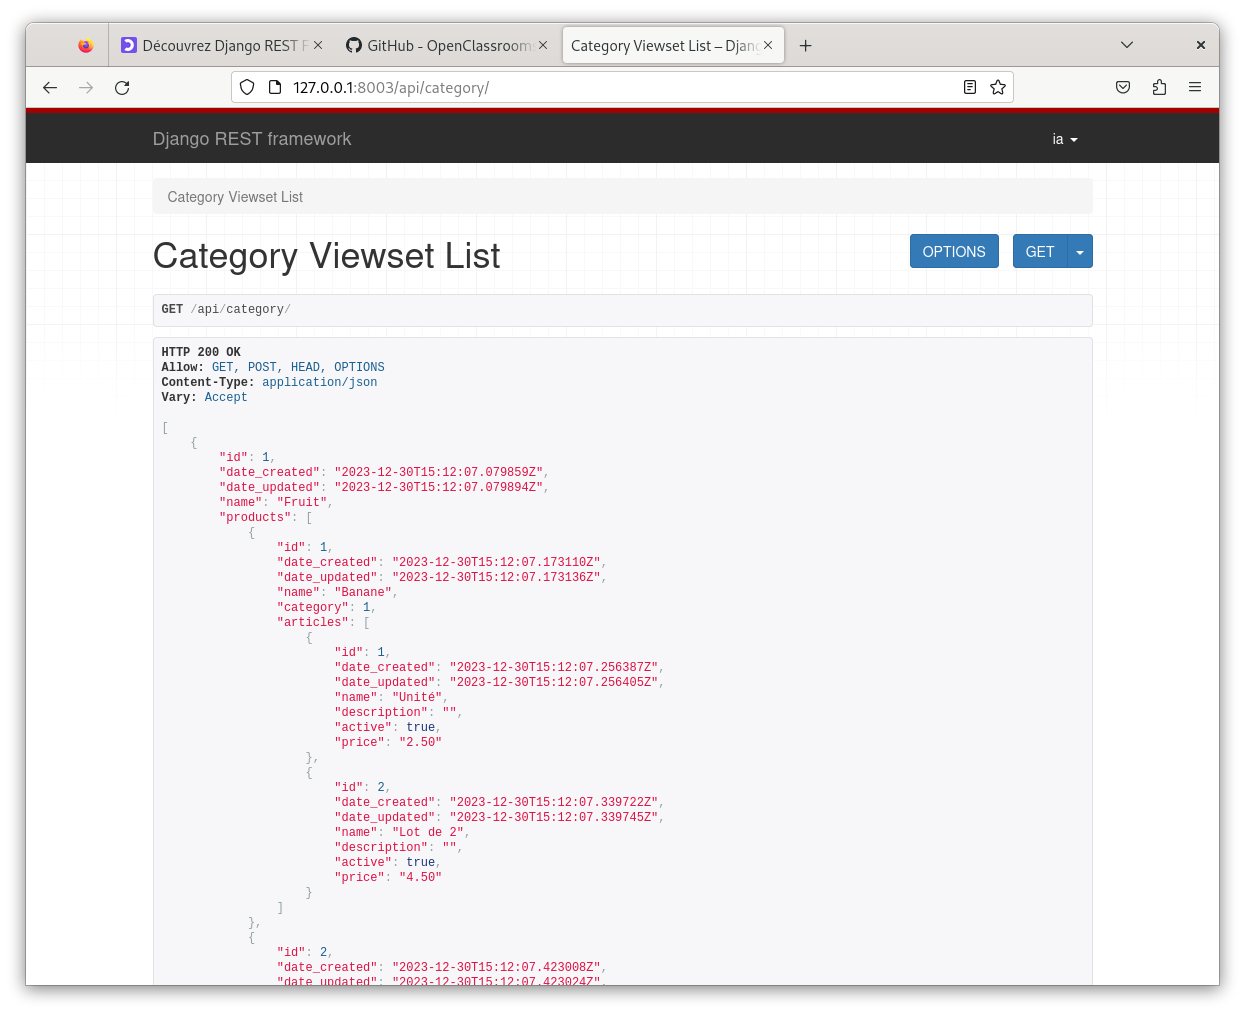
\includegraphics[width=12cm]{images/image16.png}
\end{center}
\subsubsection*{En résumé}
\begin{enumerate}
\item Imbriquer des serializers permet d’obtenir plus d’informations en un seul appel.
\item Il est possible d’appliquer des filtres sur un attribut du serializer en utilisant un {\tt SerializerMethodField}.
\item Toute modification d’un endpoint entraîne l’adaptation d’un test.
\item Il est bien de rapidement mettre en place une pagination sur une API.
\end{enumerate}

{\em Maintenant que nous avons optimisé le nombre d’appels de notre API, voyons comment différencier les informations retournées en liste ou en détail – vous me suivez au prochain chapitre ? C’est parti !}
\section{Différenciez les informations de liste et de détail}
\subsection{Retournez plus d’informations dans le détail}
Très souvent, les données en retour sont différentes selon qu’on consulte un endpoint de liste ou un endpoint de détail. En règle générale, les listes sont appelées pour être affichées. Lorsque l’utilisateur sélectionne un des éléments qui la composent, alors un autre appel est réalisé par l’application cliente afin d’obtenir plus d’informations. Cela permet de {\em réduire les temps de réponse} en ne retournant que les informations utiles.

Dans notre cas, la liste des catégories est bien trop complète pour l’usage qui doit en être fait, et nous allons donc réduire les informations de liste, en conservant toutes nos données actuelles dans l'endpoint de détail d’une catégorie.
\subsection{Améliorez le rendu du détail d’un endpoint}
Améliorons notre endpoint de catégories en ne retournant que les informations {\em minimales}, dans le cas d’une liste, et {\em détaillées}, lorsque nous consultons une catégorie spécifique.

DRF nous permet au travers de ses viewsets de redéfinir la méthode {\tt get\_serializer\_class}  qui, elle, détermine le serializer à utiliser. Par défaut, le serializer retourné est celui défini sur l’attribut de classe {\tt serializer\_class}  du viewset.

Lorsqu’une requête entre dans notre API, les viewsets définissent un attribut action  qui correspond à l’{\em action} que l’{\em application client} est en train de réaliser. Elle peut être :
\begin{itemize}
\item {\tt list :} appel en GET  sur l’URL de liste ;
\item {\tt retrieve :} appel en GET  sur l’URL de détail (qui comporte alors un identifiant) ;
\item {\tt create :} appel en POST  sur l’URL de liste ;
\item {\tt update :} appel en PUT  sur l’URL de détail ;
\item {\tt partial\_update :} appel en PATCH  sur l’URL de détail ;
\item {\tt destroy :} appel en DELETE  sur l’URL de détail.
\end{itemize}
\begin{minted}[
mathescape,
framesep=2mm,
baselinestretch=1.2,
fontsize=\footnotesize,
bgcolor=LightGray,
%linenos
]{python}
class CategoryViewset(ReadOnlyModelViewSet):
 
    serializer_class = CategoryListSerializer
    # Ajoutons un attribut de classe qui nous permet de définir notre serializer de détail
    detail_serializer_class = CategoryDetailSerializer
 
    def get_queryset(self):
        return Category.objects.filter(active=True)
 
    def get_serializer_class(self):
    # Si l'action demandée est retrieve nous retournons le serializer de détail
        if self.action == 'retrieve':
            return self.detail_serializer_class
        return super().get_serializer_class()
\end{minted}
\begin{center}
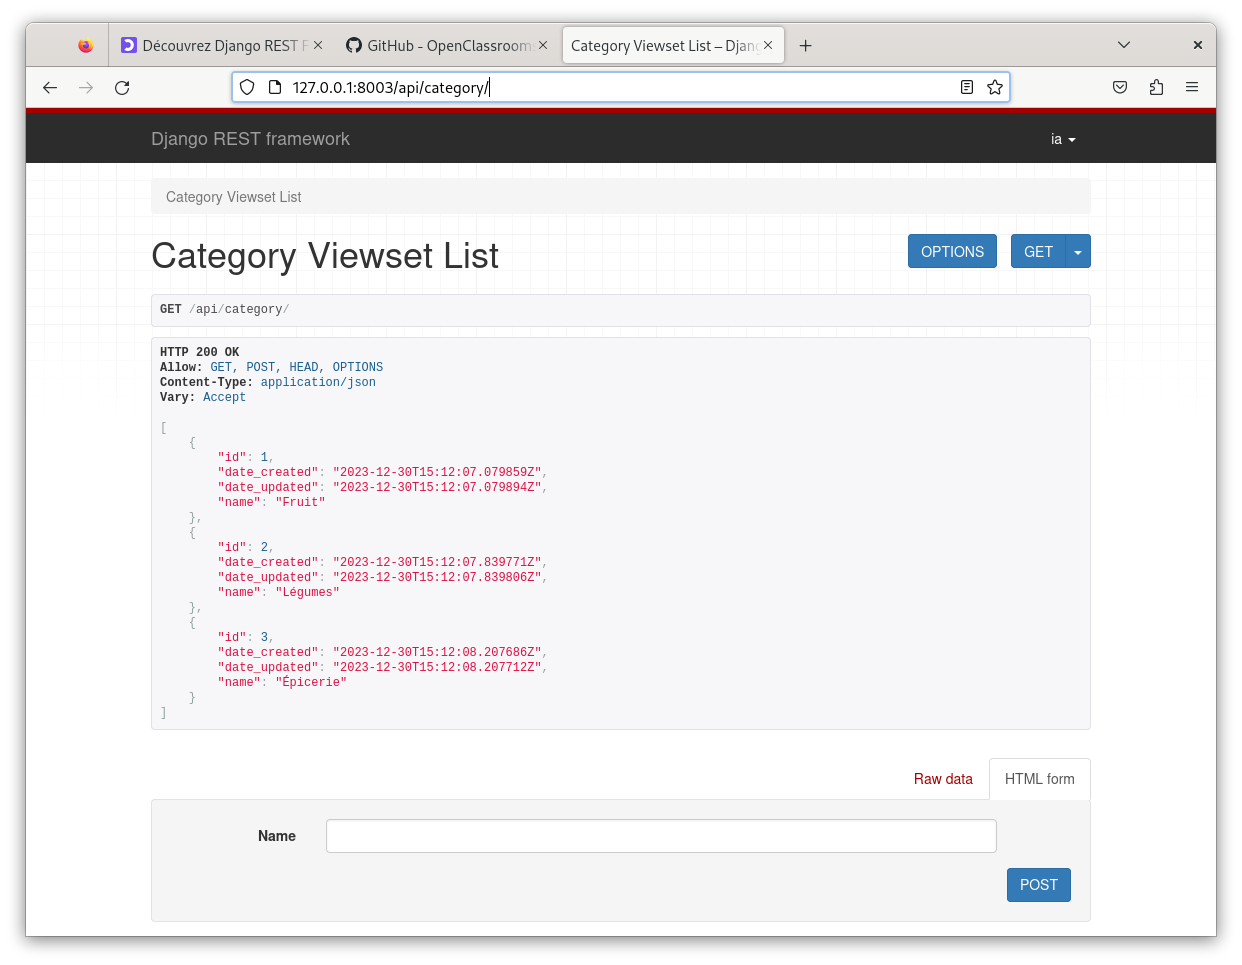
\includegraphics[width=12cm]{images/image17.png}
\end{center}
\begin{center}
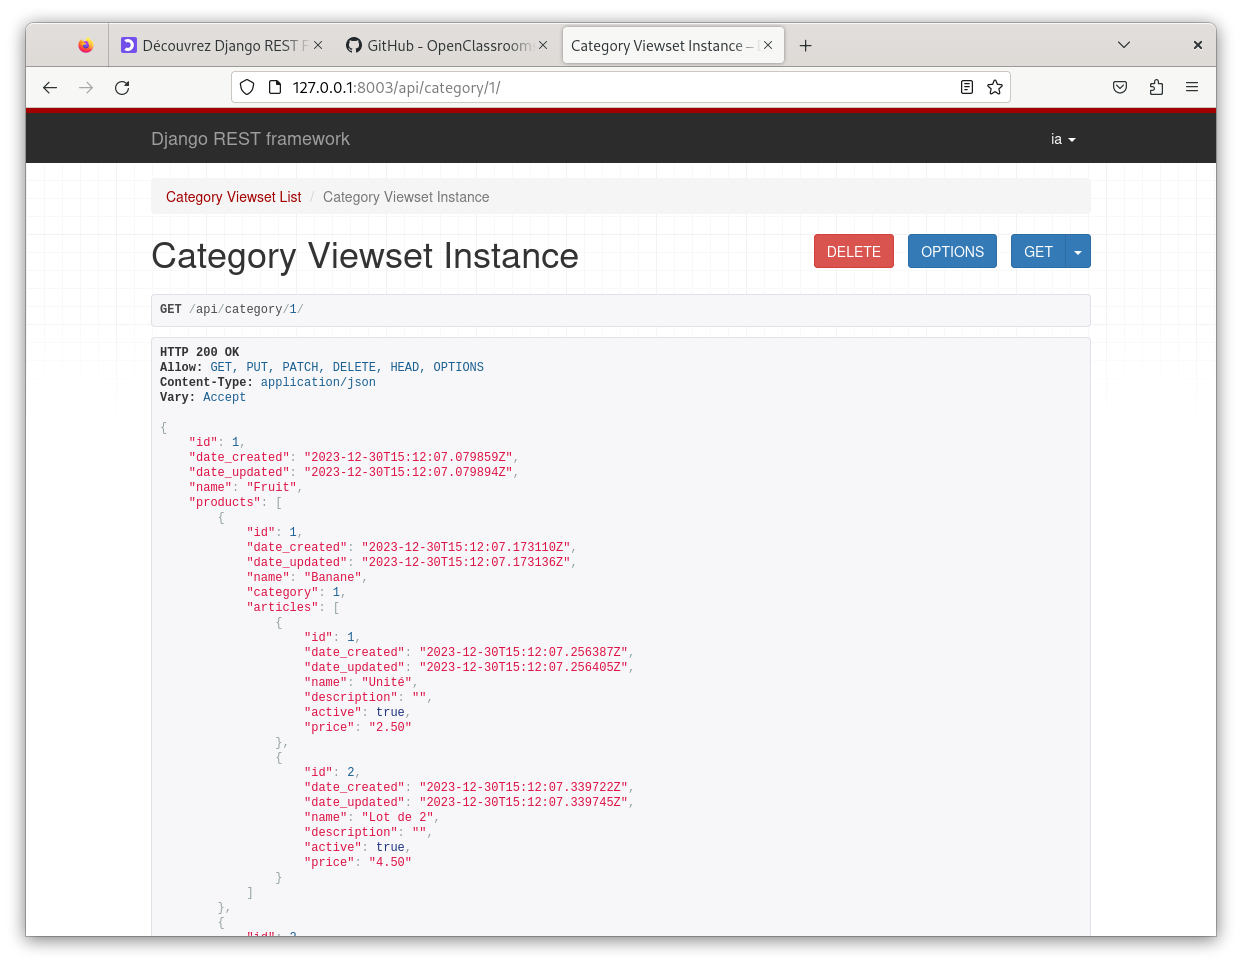
\includegraphics[width=12cm]{images/image18.png}
\end{center}

\subsubsection*{Exemple}
À vous à présent, faites de même et améliorez l'endpoint de produits pour que la liste reste succincte, et que le détail retourne plus d’informations. Pour réaliser cela, vous pouvez partir de la branche \href{https://github.com/OpenClassrooms-Student-Center/7192416\_APIs\_DRF/tree/P2C2\_exercice}{P2C2\_exercice}. Elle contient déjà ce que nous venons de faire ensemble. Une solution est proposée sur la branche \href{https://github.com/OpenClassrooms-Student-Center/7192416\_APIs\_DRF/tree/P2C1\_solution}{P2C2\_solution}.

\subsubsection*{En résumé}
\begin{enumerate}
\item L’action réalisée est définie dans l’attribut {\tt action}  des viewsets, et permet de savoir précisément l’action en cours.
\item Il est possible de définir un serializer différent pour chaque action.
\item Les mixins sont une bonne façon de gérer les différents serializers à utiliser, car cette opération est très courante.
\item Utiliser différents serializers contribue à améliorer les performances de l’API.
\end{enumerate}
{\em Dissocier les serializers de liste et de détail nous permettrait par exemple d’inclure les produits et articles dans le détail d’une catégorie. N’hésitez pas à expérimenter. }

\section{Ajoutez de l’interaction avec les actions}
\subsection{Ne soyez pas trop actif !}
\subsubsection*{Une action, on a déjà parlé de ça, non ?}
Nous avons parlé du paramètre action  des Viewsets, mais dans ce chapitre nous allons voir le {\color{monOrange}décorateur} {\tt action},  fourni par DRF, qui permet de réaliser d’autres types d’actions que les classiques du CRUD, comme {\em Demander en ami}, {\em S’abonner à un fil d’actualité} ou {\em Publier un article}.

Vous devez penser  {\color{monOrange}Action} chaque fois qu’un besoin fait référence à une entité, mais que le verbe ne correspond pas à un élément du CRUD. Par exemple, dans {\em Nous souhaitons que nos visiteurs puissent liker des publications}, l’ {\color{monOrange}entité est la publication} et l’ {\color{monOrange}action est liker}.

Une action se crée dans DRF en mettant en place le décorateur {\tt action}  sur une méthode d’un Viewset. Les paramètres suivants sont disponibles :
\begin{itemize}
\item {\tt methods}  est la liste des méthodes HTTP qui appellent cette action, parmi GET, POST, PATCH, PUT, DELETE.
\item {\tt detail}  est un booléen qui précise si l’action est disponible sur l’URL de liste ou de détail.
\item {\tt url\_path}  permet de déterminer l’URL qui sera ajoutée à la fin de l'endpoint de liste ou de détail. S'il n’est pas précisé, alors le nom de la méthode est utilisé.
\end{itemize}
Pour notre boutique en ligne, on pourrait imaginer une action qui permette d’{\color{monOrange}activer} ou de désactiver une catégorie.

\subsubsection*{Mais on ne pourrait pas juste faire un PATCH sur la catégorie pour mettre active  à False  ?}
On pourrait effectivement, mais nous aimerions également désactiver tous les produits qui composent cette catégorie. Plutôt que de laisser les applications clientes faire tous ces appels, mettons-leur à disposition {\color{monOrange}un seul endpoint} qui réalise cela. D’ailleurs, vous savez quoi ? On va le faire tout de suite… ;)
\subsection{Soyez actif quand même !}
Les actions se mettent en place sur les Viewsets, alors allons modifier notre {\tt CategoryViewset}  pour lui ajouter une action {\tt disable}  que nous souhaitons accessible en POST.
\begin{minted}[
mathescape,
framesep=2mm,
baselinestretch=1.2,
fontsize=\footnotesize,
bgcolor=LightGray,
%linenos
]{python}
 @transaction.atomic
    @action(detail=True, methods=['post'])
    def disable(self, request, pk):
        # Nous avons défini notre action accessible sur la méthode POST seulement
        # elle concerne le détail car permet de désactiver une catégorie

        # Nous avons également mis en place une transaction atomique car plusieurs requêtes vont être exécutées
        # en cas d'erreur, nous retrouverions alors l'état précédent

        # Désactivons la catégorie
        category = self.get_object()
        category.active = False
        category.save()

        # Puis désactivons les produits de cette catégorie
        category.products.update(active=False)

        # Retournons enfin une réponse (status_code=200 par défaut) pour indiquer le succès de l'action
        return Response()
\end{minted}
Ainsi, la réalisation d’un POST sur l'endpoint \href{http://127.0.0.1:8000/api/category/2/disable/}  aura pour effet de :
\begin{enumerate}
\item Désactiver la {\color{monOrange}catégorie}, ce qui ne rendra plus visible la catégorie sur l'endpointhttp://127.0.0.1:8000/api/category/.
\item Désactiver {\color{monOrange}les produits de cette catégorie}, ce qui ne rendra plus visible ces produits sur l'endpoint http://127.0.0.1:8000/api/product/.
\end{enumerate}
\begin{theorem}
Il est toujours préférable de rapprocher le code métier du model afin de pouvoir l’exécuter plus facilement. Faisons cela, et notre action en sera alors simplifiée.
\end{theorem}
Ajoutons une méthode {\tt disable}  à notre model {\tt Category}  :
\begin{minted}[
mathescape,
framesep=2mm,
baselinestretch=1.2,
fontsize=\footnotesize,
bgcolor=LightGray,
%linenos
]{python}
class Category(models.Model):
 
    date_created = models.DateTimeField(auto_now_add=True)
    date_updated = models.DateTimeField(auto_now=True)
 
    name = models.CharField(max_length=255)
    active = models.BooleanField(default=False)
 
    @transaction.atomic
    def disable(self):
        if self.active is False:
        # Ne faisons rien si la catégorie est déjà désactivée
            return
        self.active = False
        self.save()
        self.products.update(active=False)
\end{minted}
\begin{theorem}
Vous remarquerez que nous avons déplacé la transaction atomique sur la méthode du model, elle n’est donc plus nécessaire sur l’action du Viewset.
\end{theorem}
\begin{minted}[
mathescape,
framesep=2mm,
baselinestretch=1.2,
fontsize=\footnotesize,
bgcolor=LightGray,
%linenos
]{python}
class MultipleSerializerMixin:
    # Un mixin est une classe qui ne fonctionne pas de façon autonome
    # Elle permet d'ajouter des fonctionnalités aux classes qui les étendent

    detail_serializer_class = None

    def get_serializer_class(self):
        # Notre mixin détermine quel serializer à utiliser
        # même si elle ne sait pas ce que c'est ni comment l'utiliser
        if self.action == 'retrieve' and self.detail_serializer_class is not None:
            # Si l'action demandée est le détail alors nous retournons le serializer de détail
            return self.detail_serializer_class
        return super().get_serializer_class()

class CategoryViewset(MultipleSerializerMixin, ReadOnlyModelViewSet):
 
    serializer_class = CategoryListSerializer
    detail_serializer_class = CategoryDetailSerializer
 
    @action(detail=True, methods=['post'])
    def disable(self, request, pk):
        # Nous pouvons maintenant simplement appeler la méthode disable
        self.get_object().disable()
        return Response()
\end{minted}
\begin{center}
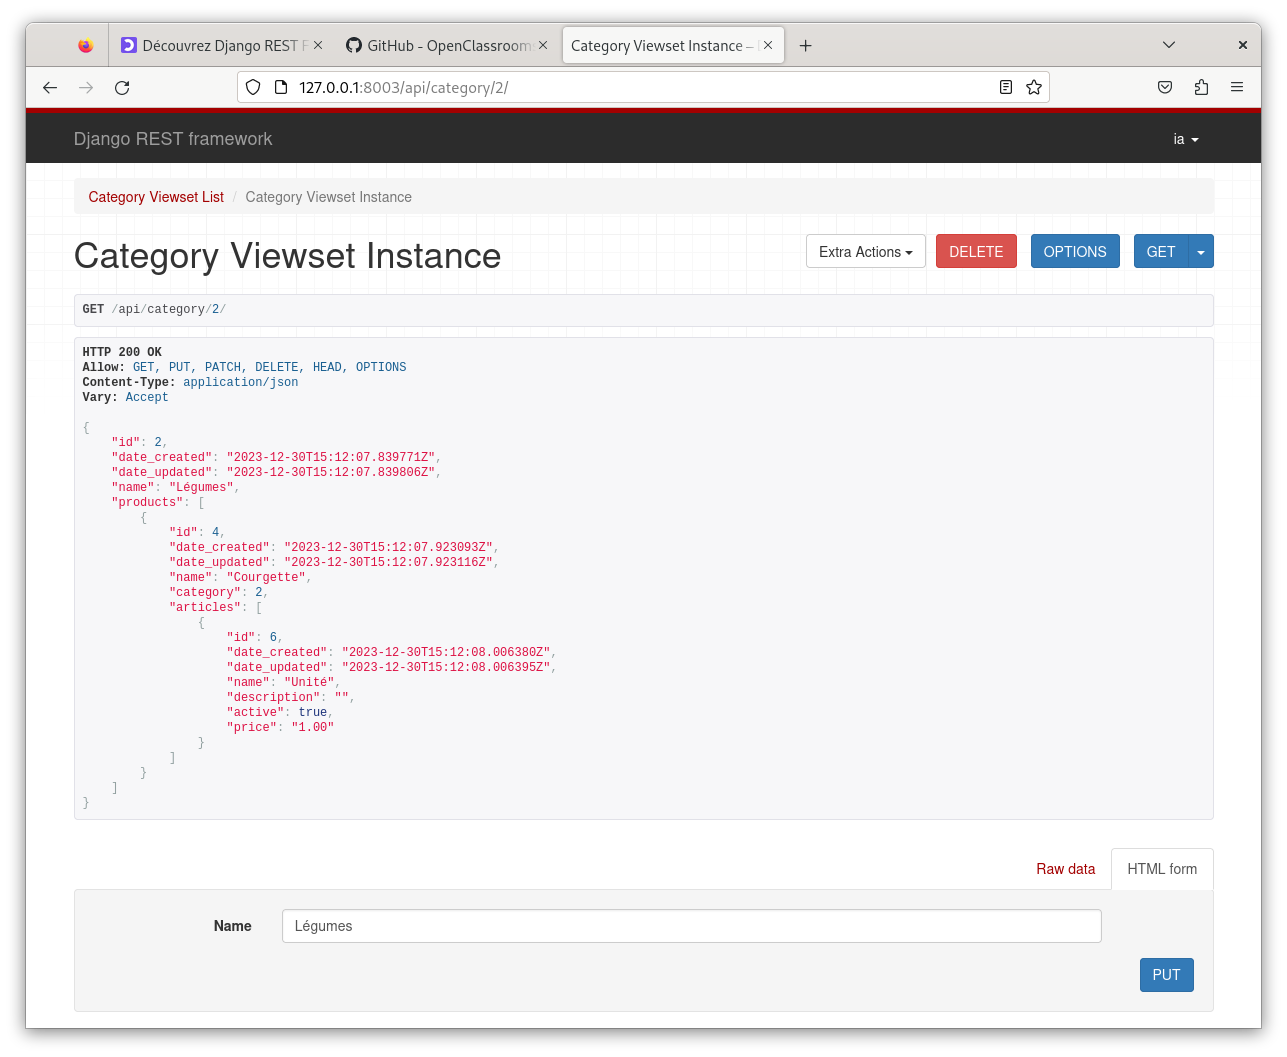
\includegraphics[width=12cm]{images/image19.png}
\end{center}
\begin{center}
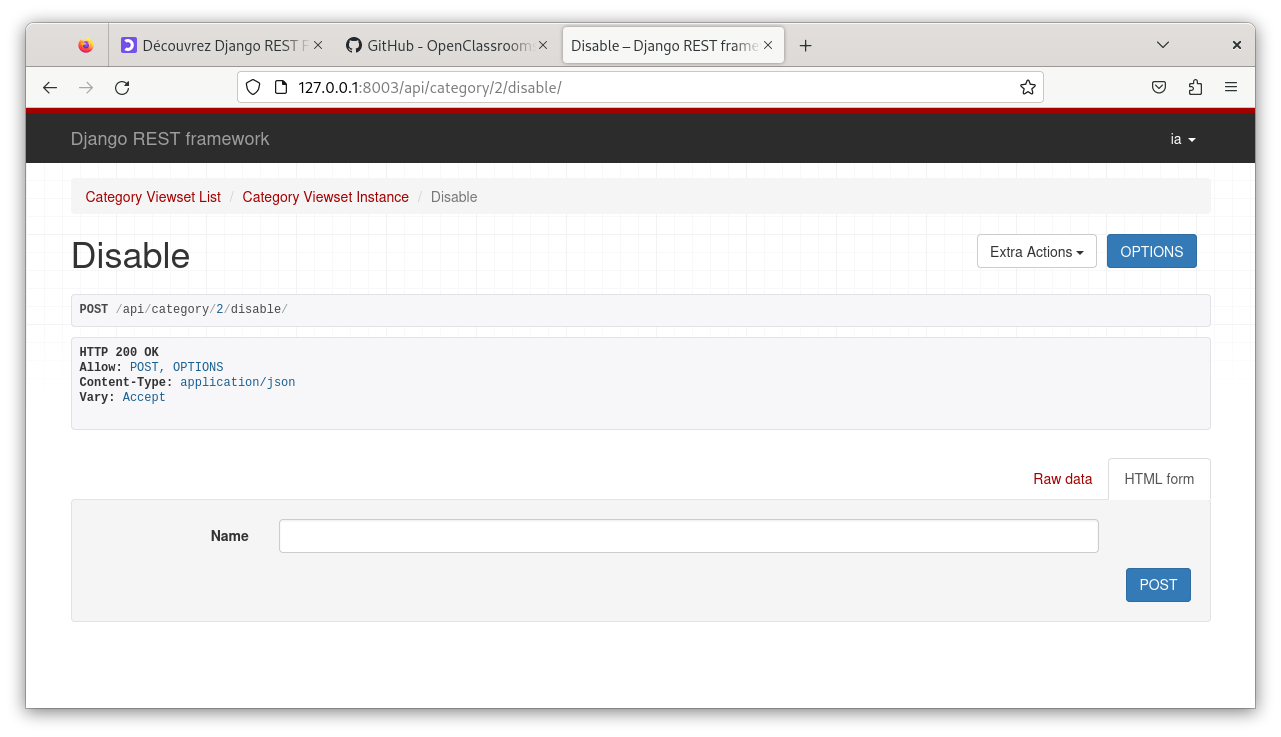
\includegraphics[width=12cm]{images/image20.png}
\end{center}


\begin{theorem}
Cette modification ne change en rien le fonctionnement de notre API, mais permet une {\color{monOrange}lecture} plus claire du code. L’action ne fait qu'appeler une méthode de notre model {\tt Category}.
\end{theorem}

\subsubsection*{Exercice}
Mettons en place le même système pour {\color{monOrange}désactiver un produit} qui {\color{monOrange}désactive également les articles associés}. Nous pourrions également améliorer la désactivation d’une catégorie en désactivant les articles de chaque produit.

Pour réaliser cela, vous pouvez partir de la branche \href{https://github.com/OpenClassrooms-Student-Center/7192416\_APIs\_DRF/tree/P2C3\_exercice}{P2C3\_exercice}. Elle contient déjà ce que nous venons de faire ensemble. Une solution est proposée sur la branche \href{https://github.com/OpenClassrooms-Student-Center/7192416\_APIs\_DRF/tree/P2C3\_solution}{P2C3\_solution}.
\subsubsection*{En résumé}
\begin{enumerate}
\item Il est possible de créer d’autres actions en dehors de celles du CRUD.
\item DRF met à disposition un décorateur {\tt action}  qui permet de créer de nouvelles actions.
\item Les actions peuvent être mises en place sur les URL de liste et de détail d’un endpoint.
\item Les actions peuvent utiliser n’importe quelle méthode HTTP (GET, POST, PATCH, DELETE…).
\end{enumerate}
{\em Les actions servent à gérer des morceaux de logique métier, et ainsi à éviter aux applications clientes de les gérer, car elles pourraient les gérer différemment. Le fait d’ajouter un article au panier d’un utilisateur est un bon exemple d’action qui ne peut être réalisé que d’une seule façon, son traitement doit donc être réalisé par le serveur et non les applications clientes. Dans le chapitre suivant, vous découvrirez comment valider les données transmises par ces actions !}

%%%%%%%%%%%%%%%%%%%%%%%%%%%%%%%%%%%%%%%%%%%%%%%
\section{Validez les données}
\subsection{Ne permettez pas la création de tout et n’importe quoi}
Attaquons-nous à présent à un autre sujet : {\color{monOrange}la création d’entités} et plus précisément de catégories, dans notre cas.

Notre endpoint actuel permet la lecture seulement, car il est destiné aux visiteurs de notre boutique. Nous allons très vite en mettre un second en place, qui sera dédié aux {\color{monOrange}administrateurs} qui, eux, auront la possibilité de {\color{monOrange}créer, modifier et supprimer} des données. La création d’entité impose d’effectuer certains contrôles qui sont généralement de deux types :
\begin{enumerate}
\item Les contrôles {\color{monOrange}sur un champ}, comme par exemple vérifier que le nom d’une catégorie n'existe pas déjà, et ainsi éviter les doublons.
\item Les contrôles {\color{monOrange}multichamps}, comme la vérification que les deux mots de passe saisis à l’inscription sont les mêmes.
\end{enumerate}
DRF nous permet de réaliser ces deux types de contrôles au travers de la réécriture de méthodes sur le serializer :
\begin{itemize}
\item {\tt validate\_XXX}  où XXX est le nom du champ à valider ;
\item {\tt validate}  qui permet un contrôle global sur tous les champs du serializer.
\end{itemize}
N’attendons pas plus longtemps pour mettre en place l'endpoint et les contrôles qui l’accompagnent. ;)

\subsection{Validez les données d’un champ}
Commençons tout de suite par la mise en place du nouvel endpoint sur l’URL \href{http://127.0.0.1:8000/api/admin/category/}  qui, comme son nom l’indique, servira à administrer les catégories.
\subsubsection*{Pourquoi ne pas utiliser l’endpoint déjà existant ?}
 Dans les endpoints d’administration :
\begin{itemize}
\item Des serializers différents sont utilisés et les données retournées diffèrent ;
\item Certains accès peuvent également être limités à certaines personnes authentifiées.
\end{itemize}
 
Dans le cadre de notre boutique, nous avons décidé de {\color{monOrange}définir nos endpoints} en fonction des {\color{monOrange}acteurs} qui les utilisent. Créons {\color{monOrange}notre nouvel endpoint d’administration} qui cette fois-ci étend {\tt ModelViewset}  et non plus {\tt ReadOnlyViewset}. Celui-ci ne doit pas avoir de limitation sur les catégories actives, car il s’agit d’un endpoint d’administration.
\begin{minted}[
mathescape,
framesep=2mm,
baselinestretch=1.2,
fontsize=\footnotesize,
bgcolor=LightGray,
%linenos
]{python}
class AdminCategoryViewset(MultipleSerializerMixin, ModelViewSet):
 
    serializer_class = CategoryListSerializer
    detail_serializer_class = CategoryDetailSerializer
 
    def get_queryset(self):
        return Category.objects.all()
\end{minted}
Puis définissons notre nouvel endpoint en le {\color{monOrange}déclarant auprès de notre routeur}.

\begin{minted}[
mathescape,
framesep=2mm,
baselinestretch=1.2,
fontsize=\footnotesize,
bgcolor=LightGray,
%linenos
]{python}
router.register('admin/category', AdminCategoryViewset, basename='admin-category')
\end{minted}
Vérifions que notre endpoint est bien fonctionnel sur l’URL  
\begin{center}
\url{http://127.0.0.1/api/admin/category}
\end{center}
Maintenant que nous utilisons un {\tt Viewset}, {\color{monOrange}la création de catégorie est possible}. C’est à la création que sert ce formulaire en nous permettant d'effectuer des actions POST. Les actions de mise à jour et de suppression sont disponibles sur les URL de détail des catégories.

Validons à présent nos données, sans oublier que la création d’un doublon de catégorie ne doit pas être permis. Il nous faut pour cela modifier notre serializer de liste, car c’est lui qui est utilisé pour l’action create  .

La {\color{monOrange}validation d’un champ} unique se fait en écrivant la méthode {\tt validate\_XXX}  où XXX  est le nom du champ. Dans notre cas, {\color{monOrange}validate\_name}  :
\begin{minted}[
mathescape,
framesep=2mm,
baselinestretch=1.2,
fontsize=\footnotesize,
bgcolor=LightGray,
%linenos
]{python}
class CategoryListSerializer(serializers.ModelSerializer):
 
    class Meta:
        model = Category
        fields = ['id', 'date_created', 'date_updated', 'name']
 
    def validate_name(self, value):
        # Nous vérifions que la catégorie existe
        if Category.objects.filter(name=value).exists():
        # En cas d'erreur, DRF nous met à disposition l'exception ValidationError
            raise serializers.ValidationError('Category already exists')
        return value
\end{minted}
Si nous tentons à présent de créer une catégorie qui existe déjà, une réponse en 400 avec des données contenant la nature de l’erreur sont renvoyées.
\begin{center}
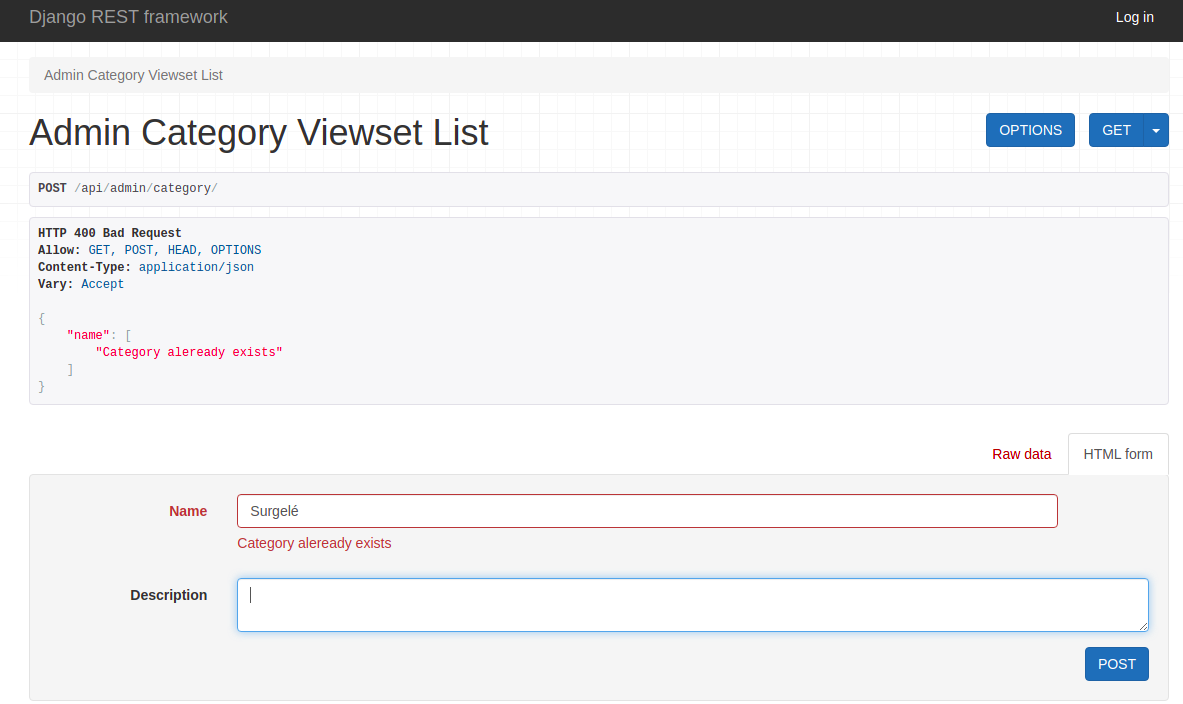
\includegraphics[width=12cm]{images/image21.png}
\end{center}
La validation de champ unique permet d’effectuer plein de {\color{monOrange}contrôles}, tant qu’ils sont effectués sur ce champ précis. On pourrait imaginer un système de filtre de mots pour un forum, par exemple.

\subsection{Mettez en place une validation multiple}
Pour notre boutique, nous souhaitons optimiser le référencement et avoir un rappel du nom de la catégorie également présent dans la description. Nous pouvons effectuer automatiquement ce contrôle au travers d’une validation multiple.

La validation entre champs se fait au travers de la méthode {\tt validate}. Vérifions que le nom est bien présent dans la description :


\begin{minted}[
mathescape,
framesep=2mm,
baselinestretch=1.2,
fontsize=\footnotesize,
bgcolor=LightGray,
%linenos
]{python}
class CategoryListSerializer(serializers.ModelSerializer):
 
    class Meta:
        model = Category
        # Pensons à ajouter « description » à notre liste de champs
        fields = ['id', 'date_created', 'date_updated', 'name', 'description']
 
    def validate_name(self, value):
        if Category.objects.filter(name=value).exists():
            raise serializers.ValidationError('Category already exists')
        return value
 
    def validate(self, data):
        # Effectuons le contrôle sur la présence du nom dans la description
        if data['name'] not in data['description']:
        # Levons une ValidationError si ça n'est pas le cas
            raise serializers.ValidationError('Name must be in description')
        return data
\end{minted}
Nous pouvons alors constater que notre validation fonctionne si le nom de la catégorie n’est pas présent dans sa description.
\begin{center}
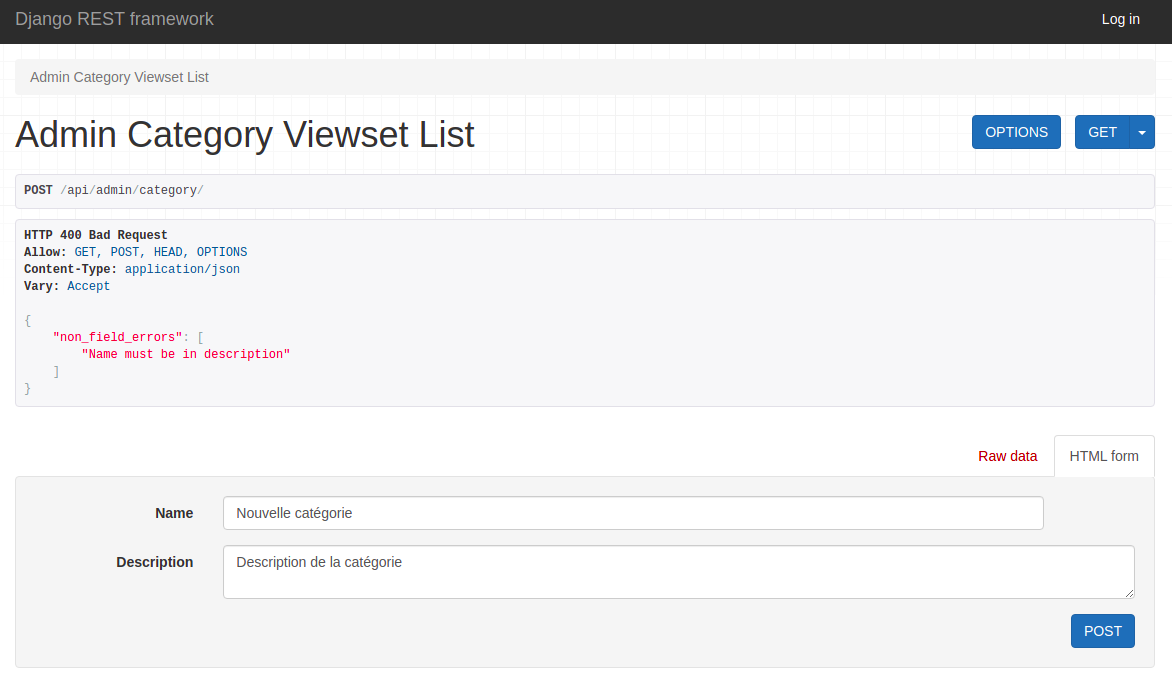
\includegraphics[width=12cm]{images/image22.png}
\end{center}

\subsubsection*{Exercice}
Mettons en place un endpoint d’administration des articles pour les administrateurs de la boutique. Certains contrôles doivent être effectués :
\begin{itemize}
\item Le {\color{monOrange}prix} doit être supérieur à 1€.
\item Le produit associé doit être {\color{monOrange}actif}.
\end{itemize}
Pour réaliser cela, vous pouvez partir de la branche \href{https://github.com/OpenClassrooms-Student-Center/7192416\_APIs\_DRF/tree/P2C4\_exercice}{P2C4\_exercice}. Elle contient déjà ce que nous venons de faire ensemble. Une solution est proposée sur la branche \href{https://github.com/OpenClassrooms-Student-Center/7192416\_APIs\_DRF/tree/P2C4\_solution}{P2C4\_solution}.

\subsubsection*{En résumé}
\begin{enumerate}
\item Utiliser un ModelViewset permet l’utilisation de l’ensemble des actions du CRUD.
\item La validation d’un champ se fait au travers de la méthode {\tt validate\_XXX}  du serializer.
\item La validation multichamp se fait au travers de la méthode {\tt validate}  du serializer.
\end{enumerate}
{\em La validation des données lors de la création et/ou la modification est un facteur clé pour assurer la cohérence des données, n’hésitez pas à valider toutes les données importantes. Maintenant, voyons comment tester les API externes avec les mocks – suivez-moi au prochain chapitre !}
\end{document}










